\chapter{Performance Investigation of the Fribourg Construction}
\label{experiment}
In this chapter we come to the core of this thesis, the empirical investigation of the performance of the Fribourg construction. Our goal is to find out how the Fribourg construction performs on real automata. In particular, we are interested mainly in two things. First, how the Fribourg construction behaves under the different optimisations that we explained in Chapter~\ref{fribourg_construction}. Second, how the Fribourg construction compares to other complementation constructions.



\section{The GOAL Tool}
\label{goal}
\subsection{Overview}
GOAL stands for Graphical Tool for Omega-Automata and Logics and has been developed at the National University of Taiwan since 2007~\cite{2007_goal,2008_goal_ext}. The tool is based on the three pillars, \om-automata, temporal logic formulas, and games. It allows to create instances of each of these notions, and manipulate them in a multitude of ways. Relevant for our purposes are the \om-automata capabilites of GOAL.

With GOAL, one can create Büchi, Muller, Rabin, Streett, parity, generalised Büchi, and co-Büchi automata, either by manually defining them, or by having them randomly generated. It is then possible to perform a plethora of operations on these automata. The entirety of provided operations are too many to list, but they include containment testing, equivalence testing, minimisation, determinisation, conversions to other \om-automata types, product, intersection, and, of course, complementation.

All this is accessible by both, a grahical and a command line interface. The graphical interface is shown in Figure~\ref{goal_gui}. Automata are displayed in the main editor window of the GUI. They can be freely edited, such as adding or removing states and transitions, and arranging the layout. There are also various layout algorithms for automatically laying out large automata. Most of the functionality provided by the graphical interface is also accessible via a command line mode. This makes it suitable for automating the execution of operations.

\begin{figure}
\begin{center}
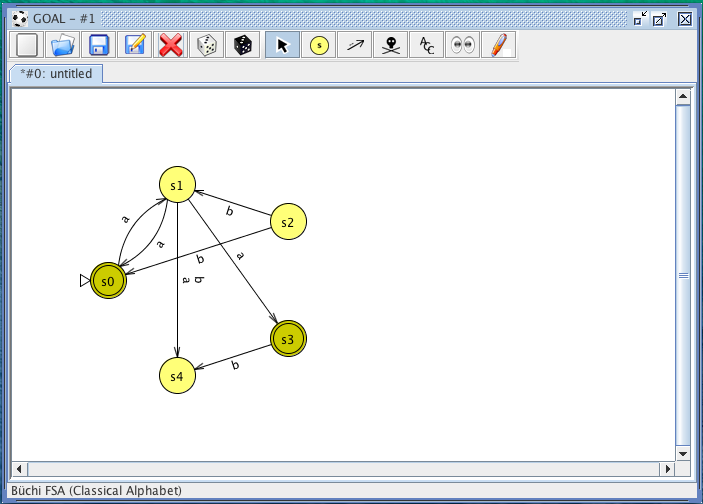
\includegraphics[scale=0.5]{figures/goal_gui.png}
\caption{Graphical interface of GOAL.}
\label{goal_gui}
\end{center}
\end{figure} 

For storing automata, GOAL defines an own XML-based file format, called GOAL File Format, usually indicated by the file extension gff.

An important design concept of GOAL is modularity. GOAL uses the Java Plugin Framework (JPF)~\footnote{http://jpf.sourceforge.net/}, a library for building modular and extensible Java applications. A JPF application defines so-called extension points for which extensions are provided. These extensions contain the actual functionality of the application. Extensions and extension points are bundled in plugins, the main building block of a JPF application. It is therefore possible to extend an existing JPF application by bundling a couple of new extensions for existing extensions points in a new plugin, and installing this plugin into the existing application. On the next start of the application, the new functionality will be included, all without requring to recompile the existing application or to even have its source code.

GOAL provides a couple of extensions points, such as \textit{Codec}, \textit{Layout}, or \textit{Complementation Construction}. An extension for \textit{Codec}, for example, allows to add the handling of a new file format which GOAL can read from and write to. With an extension for \textit{Layout} one can add a new layout algorithm for laying out automata in the graphical interface. And an extension to \textsf{Complementation Construction} allows to add a new complementation construction to GOAL. This is how we added the Fribourg construction to GOAL, as we will further explain in Section~\ref{implementation}.

\subsection{Büchi Complementation}
There are a couple of Büchi complementation constructions preimplemented in GOAL. Table~\ref{goal_constructions} summarises them, showing for each one its name on the graphical interface and in the command line mode, and the reference to the paper introducing it. As can be seen, the most important representants of all the four approaches (Ramsey-based, determinisation-based, rank-based, and slice-based, see Chapter~\ref{background}) are present. Note that in addition to the listed constructions, GOAL also contains Kurshan's construction and classic complementation. These are for complementing DBW and NFA/DFA, respectively, and thus not relevant to us.

\begin{table}
\caption{The complementation constructions implemented in GOAL (version 2014-11-17).}
\begin{center}
\begin{tabular}{|l|l|l|}
\hline
Name & Command line & Reference \\
\hline
Ramsey-based construction & ramsey & Sistla, Vardi, Wolper (1987)~\cite{PrasadSistla1987217} \\
\hline
Safra's construction & safra & Safra (1988)~\cite{1988_safra_1} \\
\hline
Modified Safra's construction & modfiedsafra & Althoff (2006)~\cite{2006_althoff} \\
\hline
Muller-Schupp construction & ms & Muller, Schupp (1995)~\cite{Muller199569} \\
\hline
Safra-Piterman construction & piterman & Piterman (2007)~\cite{2007_piterman} \\
\hline
Via weak alternating parity automaton & wapa & Thomas (1999)~\cite{1999_thomas} \\
\hline
Via weak alternating automaton & waa & Kupferman, Vardi (2001) \cite{Kupferman:2001} \\
\hline
Rank-based construction & rank & Schewe (2009) \cite{schewe2009buchi} \\
\hline
Slice-based construction (preliminary) & slice -p & Vardi, Wilke (2007) \cite{vardi2007automata} \\
\hline
Slice-based construction & slice & Kähler, Wilke (2008) \cite{2008_kaehler} \\
\hline
\end{tabular}
\end{center}
\label{goal_constructions}
\end{table}

Complementation constructions in GOAL can define a set of options that can be set by the user. In the graphical interface this is done via a dialog window, in the command line mode via command line arguments. Figure~\ref{goal_complementation_options} shows the options dialog of the Safra-Piterman construction. Complementation options allow to play with different configurations and variants of a construction, and we will make use of them for including the optimsations presented in Chapter~\ref{fribourg_construction} to the implementation of the Fribourg construction.


\begin{figure}
\begin{center}
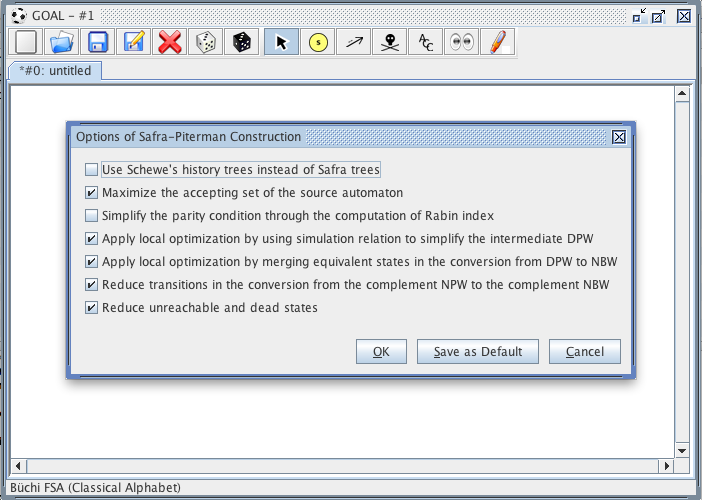
\includegraphics[scale=0.5]{figures/goal_complementation_options.png}
\caption{Complementation constructions in GOAL can have a set user-selectable options. Here the options of the Safra-Piterman construction.}
\label{goal_complementation_options}
\end{center}
\end{figure}

For most complementation constructions (all listed in Table~\ref{goal_constructions} except the Ramsey-based construction) there is also a step-by-step execution version.


\section{Implementation of the Fribourg Construction}
\label{implementation}

\section{Experiment Idea}
\label{experiment_idea}

\section{Experiment Setup}
\label{experiment_setup}